\chapter{Форми HTML. Змінні, константи, масиви та функції в РНР}
\section*{Мета роботи}
Згадати основи мови розмітки веб-сторінок. Ознайомитись з базовими елементами мови РНР.
\nopagebreak[4]
\section{Формування HTML-сторінки засобами PHP}
\nopagebreak[4]
Код PHP зазвичай об'єднується з тегами XHTML. PHP є вбудовуваним мовою~--- це означає, що можна переміщатися між чистим кодом HTML і PHP, не жертвуючи можливістю читання тексту.
\index{PHP!теги відкриття/закриття}Щоб вбудувати код PHP в XHTML, PHP повинен задаватися відокремлено, за допомогою початкового та кінцевого тегів PHP. Теги PHP кажуть інтерпретатору, де починається і закінчується код PHP. Аналізатор PHP розпізнає три варіанти початкового і кінцевого тегів.

\begin{enumerate}



\item Перший варіант тегів PHP називається тегами в стилі XML і є кращим стилем. Він працює в документах розширювана мова розмітки (XML). Цей метод повинен використовуватися при з'єднанні PHP з документами XML і XHTML. Приклади в цьому підручнику застосовують цей формат тегів XML.

Стиль XML
\begin{verbatim}
<? PHP
//Блок коду PHP
>
\end{verbatim}

    
\item Скорочений стиль є найбільш простим, однак, він не рекомендується, тому що вступає в протиріччя зі стандартами документів XML та налаштуваннями в <<php.ini>>.

Скорочений стиль    
\begin{verbatim}
<?
//Блок коду PHP
>
\end{verbatim}

    
\item Цей стиль використовує найдовшу запис і схожий на стиль тегів, що застосовуються для включення кодів JavaScript. Цей стиль є кращим при використанні редактора HTML, який не розпізнає інші стилі тегів. Так як більшість нових редакторів XHTML розпізнають стиль тегів XML, то використання цього стилю не рекомендується.

Стиль сценарію
\begin{verbatim}
<script language="php">
//Блок коду PHP
</ SCRIPT>
\end{verbatim}
   
\end{enumerate}

PHP містить два основних оператора для виведення тексту в веб-браузері: \verb|echo| і  \verb|print|. Обидва оператора розміщуються між відкритим і закритим тегами блоку коду PHP і можуть перебувати в будь-якому місці в документах XHTML. Оператори  \verb|echo| і  \verb|print| використовують наступний формат:
\verb|echo|~--- використовується для виведення одного або кількох рядків.
\begin{verbatim}
echo "виведений текст";
\end{verbatim}
 \verb|print|~--- використовується для виведення рядка. В деяких випадках оператор  \verb|print| пропонує більшу функціональність, ніж оператор  \verb|echo|.
\begin{verbatim}
print "виведений текст";
\end{verbatim}
Наступні приклади демонструють використання і розміщення команд  \verb|echo| і  \verb|print| в документі XHTML.



\begin{lstlisting}[caption=Приклад вживання команд echo і print]
<!DOCTYPE html PUBLIC "-//W3C//DTD/XHTML 1.0 Transitional//EN"
  "http://www.w3.org/TR/xhtml1/DTD/xhtml11-transitional.dtd">
<html xmlns="http://www.w3.org/1999/xhtml" xml:lang="en" lang="en">
<head>
  <title> Страница Web </title>
</head>
<body>
<?php 
echo "Друк рядка оператором echo"."<br>";
print "Друк рядка оператором print";
?>
</body>
</html>
\end{lstlisting}



\pagebreak[3]
\section{Передача даних з HTML-форми PHP-сценарію}
\nopagebreak[4]
\index{HTML!передача данних}
Обробка форм є дуже важливою властивістю PHP. За допомогою форм користувачі взаємодіють зі сторінками Web, і з їхньою ж допомогою можна збирати інформацію для персоналізованих сторінок відвідувачів. У більш широкому сенсі інформаційної обробки, форми призначені для введення даних в системи обробки. Вони є первинним механізмом отримання даних, які обробляють сценарії для породження нової інформації, поновлення файлів і баз даних, а також для відповіді на запити користувачів для отримання інформації. Зовнішній вигляд типової форми дано на малюнку~\ref{f2-1:image}.

Передача даних з форм в РНР-сценарій відбувається методами  \verb|GET| або  \verb|POST| протоколу НТТР. Обидва методи однаково ефективні при використанні в формах з невеликою кількістю полів. Метод  \verb|POST| рекомендований при передачі великих обсягів тексту і файлів, обмеження за замовчуванням встановлено в 8 Мбайт і налаштовується у файлі  \verb|php.ini|.

Контейнер форми виглядає наступним чином:
\begin{verbatim}
<form name="form1" action="script.php" method="post">
</form>
\end{verbatim}
де \verb'name'~--- назва HTML-об'єкта, \verb'action' - відносний або абсолютний шлях до сценарію, якому передаються дані, \verb'method' - назва методу, яким передаються дані.

У контейнер форми поміщаються додаткові елементи управління, якими управляє користувач:

\subsection*{INPUT і його варіації}
\index{HTML!форми!input}
Елемент \verb'<input>' є найбільш вживаним тегом HTML-форм. За допомогою цього тега реалізуються основні функції форми. Він дозволяє створювати всередині форми поля введення рядка тексту, імені файлу, пароля і т.д. Також варто згадати про варіацію тега, що реалізує можливість завантаження файлів на сервер. Повний опис можливостей даного тега дано у додатку~\ref{inp-tag:app}
\subsection*{TEXTAREA}
\index{HTML!форми!textarea}
Елемент \verb'<textarea>' відповідає за передачу багаторядкового тексту. Важливо пам'ятати, що об'єм тексту, що передається обмежений параметрами методу, який використовується для передачі. Повний опис можливостей даного тега дано у додатку~\ref{tar-tag:app}
\subsection*{Списки вибору SELECT}
\index{HTML!форми!select}
Досить часто існує необхідність представити які-небудь дані у вигляді списку і передбачити можливість вибору в цьому списку. У HTML списки реалізуються за допомогою тега \verb'<select>'. Списки можуть давати можливість одиночного або множинного вибору. Повний опис можливостей даного тега дано у додатку~\ref{sel-tag:app}

\begin{figure}
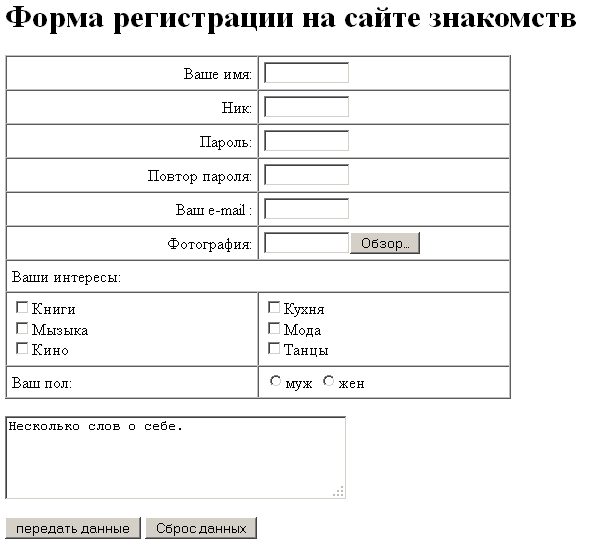
\includegraphics[scale=1,width=8cm]{ch02-01.png}
\caption{Вигляд HTML-форми}
\label{f2-1:image}
\end{figure}


\pagebreak[3]
\section{Змінні, константи та функції в РНР}
\nopagebreak[4]
\subsection*{Змінні}
\index{PHP!змінні}
\textbf{Змінні} є тимчасовим місцем зберігання, використовуваним для представлення значень в сценарії PHP. У PHP є два основні типи змінних: скалярні і масиви. Скалярні змінні містять тільки одне значення в даний момент часу, а змінні масиви - список значень. Змінні масиви обговорюються в наступному розділі. Скалярні змінні PHP містять значення типів описаних у лабораторній роботі №~\ref{datatypes}.

Імена змінних PHP всіх типів починаються зі знака <<\$>>. Імена змінних можуть містити літери, числа, і символ підкреслення (\_); вони не можуть, проте, починатися з цифри. У PHP імена змінних розрізняють регістр символів. 

\subsection*{Інтерполяція змінних}
\index{PHP!змінні!інтерполяція}
PHP підтримує також процес, званий інтерполяцією. \textbf{Інтерполяція}~--- заміна змінної в рядку її вмістом. Замість з'єднання змінних і літералів, їх можна об'єднувати всередині подвійних лапок (""). Змінні і літерали не можна об'єднати всередині одиночних лапок. При використанні подвійних лапок значення змінної виводиться разом з літералів. 
\begin{verbatim}
<?php 
$fname = "John";
$lname = "Doe";
echo "The user's name is $fname $lname";
?>
\end{verbatim}
\subsection*{Константи}
\index{PHP!константи}
\textbf{Константи}, як і змінні, є тимчасовим сховищем значень у пам'яті. На відміну від змінних значення константи ніколи не змінюється. При оголошенні константи використовується функція  \verb|define()|, яка вимагає задати ім'я константи і значення цієї константи.

Константам можна присвоювати такі типи даних.

Цілі~--- цілі числа або числа без десяткової крапки (1, 999, 325 812 841).

Числа з плаваючою точкою~--- числа, що містять десяткову крапку (1.11, 2.5, .44).

Рядки~--- текстова або числова інформація. Строкові дані завжди полягають в лапки ("Hello World", "478-477-5555").

Імена констант PHP на відміну від змінних не починаються зі знака <<\$>>. Імена констант звичайно записують у верхньому регістрі. Імена констант можуть містити літери, цифри та символ підкреслення (\_); вони не можуть, проте, починатися з цифри. Оголошення констант показано нижче.
\begin{verbatim}
define ("STRING_CONSTANT", "This is my string."); 
define ("NUMERIC_CONSTANT", 5); 
\end{verbatim}
Вивід констант подібний до виводу змінних.
\subsection*{Функції}
\index{PHP!функції}
\textbf{Функцією} називається фрагмент програмного коду, що володіє унікальним ім'ям і призначений для вирішення певного завдання. 

Функції використовуються для розбиття великих блоків коду на менші, більш керовані одиниці. Код, що міститься всередині функції, виконує певне завдання і повертає значення. PHP містить два типи функцій~--- визначені користувачем (або створені програмістом) і внутрішні (вбудовані функції), які є частиною визначення мови PHP.

Виклик вбудованої функції відбувається за допомогою її імені. Наприклад, функція, що виводить інформацію про РНР та Apache:
\begin{verbatim}
<?php
phpinfo();
?>
\end{verbatim}
У даному випадку функція викликається без параметрів. Наступна функція використовує ряд аргументів і повертає значення (у даному випадку дескриптор відкритого файлу:
\begin{verbatim}
<?php
f=fopen("d:\www\index.php","w+");
?>
\end{verbatim}
\pagebreak[3]
\section{Робота з масивами в РНР}
\nopagebreak[4]
\index{PHP!змінні!масиви}
Змінну масиву можна використовувати для зберігання множини або послідовності значень. Система PHP підтримує масиви з числовими індексами і асоціативні масиви. \textbf{Масив} в PHP є фактично впорядкованим відображенням. Відображення є типом, який відображає значення в ключі. Змінні масивів складаються з двох частин~--- індексу та елемента. Індекс масиву, іноді званий ключем масиву, є значенням, застосовуваним для ідентифікації або доступу до елементів масиву. Індекс масиву поміщається в квадратні дужки. Більшість масивів використовують числові індекси, які зазвичай починаються з 0 або 1. У PHP асоціативні масиви можуть використовувати рядкові індекси. Обидва типи масивів створюються за допомогою конструкції  \verb|array()|
\subsection*{Масиви з числовими індексами}
\begin{verbatim}
$my_array = array('red', 'green', 'blue'); 
\end{verbatim}
Цей код створює масив з числовим індексом з ім'ям \verb'$my_array'. Масиву присвоюється три елементи~---  \verb|red|,  \verb|green| і  \verb|blue|. Кожен елемент ідентифікується числовим індексом.
\begin{verbatim}
$my_array [0] = 'red' // індекс 0 відповідає елементу red 
$my_array [1] = 'green' // індекс 1 відповідає елементу green 
$my_array [2] = 'blue' // індекс 2 відповідає елементу blue 
\end{verbatim}
Щоб отримати доступ до вмісту масиву, використовується ім'я масиву та індекс. 
\subsection*{Асоціативні масиви}
Асоціативні масиви дозволяють використовувати більш корисні значення індексу. Для масивів з числовими індексами значення індексу створюються автоматично, починаючи з 0. Асоціативні масиви допускають застосування числових і строкових значень індексу.
\begin{verbatim}
$members = array('FName' => 'John', 'LName' => 'Smith', 'Age' => 50) 
\end{verbatim}
У цьому прикладі члени масиву містять три елементи, однак використовуються рядкові індекси~---  \verb|FName|,  \verb|LName| і  \verb|Age|.
\begin{verbatim}
$members ['FName'] = 'John' // індекс FName відповідає елементу John
$members ['LName'] = 'Smith' // індекс LName відповідає елементу Smith
$members ['Age'] = '50 '// індекс Age відповідає елементу 50 
\end{verbatim}
Для доступу до вмісту масиву використовується ім'я масиву та індекс.
\pagebreak[3]
\section{Функції, визначені користувачем}
\nopagebreak[4]
\index{PHP!функції!користувацькі функції}
\textbf{Визначені користувачем функції} створюються за допомогою ключового слова \verb'function'. Вони особливо корисні у великих програмах PHP, так як можуть містити блоки коду, які можуть використовуватися в програмі, що дозволяє уникнути повторного переписування коду. Далі представлений приклад простої визначеної користувачем функції PHP:
\begin{verbatim}
function AddNumbers ($num1, $num2)
{
echo "Це приклад функції PHP. 
Вона обчислює суму двох чисел і повертає 
результат програмі, що її викликала";
return $num1 + $num2;
} 
\end{verbatim}


Визначені користувачем функції можуть викликатися в будь-якому місці програми на PHP. У PHP функція виконується при використанні в коді її імені. Після виклику функція отримує всі передані їй значення у формі параметрів, виконує певні завдання і повертає значення програмі. 

\pagebreak[3]
\section{Змінні всередині функції}
\nopagebreak[4]
\index{PHP!змінні!локальні змінні}
\index{PHP!змінні!глобальні змінні}
\textbf{Глобальні змінні}~--- це змінні, які доступні всій програмі, включаючи підпрограми (користувальницькі функції).

\textbf{Локальні змінні}~--- змінні, визначені всередині підпрограми (користувацької функції). Вони доступні тільки всередині функції, в якій вони визначені.

Для PHP всі оголошені і використовувані у функції змінні за замовчуванням локальні для функції. Тобто, за умовчанням немає можливості змінити значення глобальної змінної в тілі функції. 

існує спеціальна інструкція \verb'global', що дозволяє функції користувача працювати з глобальними змінними. Розглянемо даний принцип на конкретному прикладі:

\begin{verbatim}
<?php
$a = 1 ;
$b = 2 ;

function sum()
{
global $a, $b;
$b = $a + $b;
}
?> 
\end{verbatim}

\pagebreak[3]
\section{Змінні-функції}
\nopagebreak[4]
\index{PHP!функції!змінні-функції}
PHP підтримує концепцію \textbf{змінних-функцій}. Це означає, що якщо до імені змінної приєднані круглі дужки, PHP шукає функцію з тим же ім'ям, що і результат обчислення змінної, і намагається її виконати. Цю можливість можна використовувати для реалізації зворотних викликів, таблиць функцій і безлічі інших речей.

Приклад використання змінної-функції наведено в додатку~\ref{var-func:app}

\pagebreak[3]
\section{Індивідуальне завдання}

\nopagebreak[4]
\subsection*{Завдання до лабораторної роботи}
\nopagebreak[4]
\begin{enumerate}
\item Вивчити теоретичний матеріал
\item Відповісти на контрольні запитання
\item Скласти алгоритм (блок-схему) програми
\item Виконати практичне завдання
\item Скласти звіт
\item Захистити роботу
\end{enumerate}

\subsection*{Контрольні запитання}
\nopagebreak[4]
\begin{enumerate}
\item Що таке змінні, константи та функції?
\item Що таке інтерполяція змінних?
\item Що таке масиви?
\item Як отримати доступ до індексного масиву? 
\item До ассоціативного?
\item Як створити користувацьку функцію?
\item Що таке локальні змінні?
\item Що таке глобальні змінні? Як ними користуватись у тілі функції?
\item Що таке змінні-функції?
\item Яким чином здійснюється виклик функції-змінної?
\end{enumerate}

\subsection*{Практичні завдання}
\nopagebreak[4]


\begin{enumerate}
\item[]Написати HTML-сторінку з формою, що складається з:
\item однорядкового поля вводу, поля вводу пароля та кнопки відправлення форми.
\item однорядкового поля вводу, прихованого текстового поля та кнопки відправлення форми.
\item однорядкового поля вводу, багаторядкового поля вводу та кнопки відправлення форми.
\item багаторядкового поля вводу, списку з одиночним вибором з п'яти елементів та кнопки відправлення форми.
\item прихованого текстового поля, списку з одиночним вибором з п'яти елементів та кнопки відправлення форми.
\item багаторядкового поля вводу, списку з множинним вибором з п'яти елементів та кнопки відправлення форми.
\item списку з одиночним вибором з п'яти елементів, поля вводу пароля та кнопки відправлення форми.
\item списку з множинним вибором з п'яти елементів, багаторядкового поля вводу та кнопки відправлення форми.
\item[]Отримати дані форми і вивести іх за допомогою функції в окремому сценарії.
\item створити асоціативний масив з днями тижня та вивести його на сторінку
\item створити індексний массив з назвами місяців і вивести його на екран
\item[]Написати HTML-сторінку з формою, що складається з однорядкового поля вводу та кнопки відправлення. Записати в поле число та обробити наступним чином:
\item створити константу та помножити на отримане з форми число 
\item створити змінну, занести в неї результат з форми, помножити змінну саму на себе
\item створити константу та обчислити вираз $x*const+2*x$
\item створити константу та обчислити вираз $\frac{x}{const}+x^2$
\item створити змінну та константу, в змінну занести константу і додати до числа з форми.
\item[]Результат вивести на сторінку 
\item[]Створити форму з трьома однорядковими полями і кнопкою відправлення форми
\item отримані з форми дані занести в асоціативний масив
\item отримані дані занести в індексний масив
\item[]зміст масиву роздрукувати функцією \verb'print_r()'; 
\item створити функцію, що друкує свій параметр
\item створити функцію, що перемножує два свої параметри і повертає результат. Результат роздрукувати
\item створити функцію, що перемножує свої параметри і друкує результат
\item створити функцію, що змінює глобальну змінну
\item створити функцію, що перемножує глобальну змінну і вхідний параметр, рузультат друкує
\item створити функцію, що домножує глобальну змінну на вхідний параметр і повертає результат
\item створити функцію, що формує індексний масив з двох локальних змінних і друкує його функцією \verb'print_r()';
\item створити функцію, що формує асоціативний масив з параметрів і друкує його функцією \verb'print_r()';

\end{enumerate}



